\chapter{Object Reconstruction}
\label{sec:object_reconstruction}

This chapter will overview the methods used to reconstruct the objects in each event, that are critical for the searches described in Chapters~\ref{sec:bsm_H_to_tau_tau_analysis} and~\ref{sec:H_A_to_4_tau_analysis}.
The topics discussed here are the reconstruction of tracks and vertices, the particle flow algorithm, the calculation of the \ac{MET}, the measurements of jets and the tagging of their flavours, and the identification of electrons, muons, and tau leptons.

\section{Tracks and vertices}

The reconstructed vertex with the largest value of summed physics-object $\pT^{2}$ is taken to be the primary proton-proton interaction vertex. 
The physics objects for this purpose are the jets, clustered using the jet finding algorithm~\cite{Cacciari:2008gp,Cacciari:2011ma}, as described below, with the tracks assigned to the vertex as inputs, and the
associated missing transverse momentum, taken as the negative vector sum of the $\pT$ of those jets.
Any other collision vertices in the event are associated with additional soft inelastic pp collisions called \emph{pileup}.



\section{Particle flow}

The particle-flow (PF) algorithm reconstructs the products of the LHC pp collisions and is described in full in Ref.\cite{PF_CMS}.  
It utilises all the information available from the tracker, ECAL, HCAL and muon detectors combined to produce a list of particle candidates. 
These candidates are either a photon, electron, muon or a neutral or charged hadrons. It begins with defining an event as the data taken per bunch crossing. 
The PF algorithm then reconstructs the tracks of the particle candidates in order to find the collision vertices. 
The primary collision vertex is taken to be the one with the largest value of \(p_T^{2}\) summed over all physics objects originated from that vertex. 
Physics objects are not only defined to include particle candidate tracks, but also missing tracks represented by the negative vectorial sum of all particle candidate tracks. Other pp collisions vertices are referred to as pileup. \\

In reconstructing electron and muons, the energy deposits in the ECAL and the track hits in the muon chamber respectively, working alongside the tracker, provide the basis of electron and muon identification. However, additional requirements are used to drop misidentification rates by ensuring that the electron or muon is isolated from any hadronic activity in the detector, as leptons do not carry colour charge. This is done by defining a relative isolation variable \(I_{rel}^{e(\mu)}\) in the following way

\begin{equation}
    I_{rel}^{e\mu} = \frac{\sum p_{T,i} + \sum E_{T,i}}{p_T^{e\mu}}.
\end{equation}

The sums are over all particles included in a cone of radius \(\Delta R = \sqrt{(\Delta \eta)^2 + (\Delta \phi)^2}\) excluding the electron or muon itself. \(\Delta \eta\) and \(\Delta \phi\) are the angular distance in \(\eta\) and \(\phi\) around the electron or muon direction from the primary vertex. To remove problems with pileup, only charged particles originating from the primary vertex are included. To remove neutral particles from pileup in the cone, the \(p_T\) for neutral particles is estimated by subtracting half of the sum of the \(p_T\) of charged particle in the cone, due to the approximate ratio of charged to neutral hadron production. The cone size selected for electrons is \(\Delta R<0.3\) and the isolation variable is \(I_{\text{rel}}^{e(\mu)} < 0.1\). For muons is cone size is \(\Delta R<0.4\) and the isolation variable is \(I_{\text{rel}}^{e(\mu)} < 0.15\). \\

Jets originating from the hadronisation of b quarks, are identified using the combined secondary vertex b-tagging algorithm. This discriminates between jets originating from b quarks from other jets, utilising track impact parameters and secondary vertex related variables \cite{CMS_btag}. This plays a key part in the analysis, as b-tagging is used for categorisation purposes described in Section \ref{sec:cat_and_sig}. The missing transverse momentum, \(\vec{p}_T^{\hspace{1ex}\text{miss}}\), is also used in categorisation of events and is calculated as the negative vector sum of all PF reconstructed transverse momenta.

\section{Muons}

Muons are required to be reconstructed as muon by the particle flow reconstruction. They additionally must pass \textit{Medium muon} requirements~\cite{cmsMediumMuon}, 
as recommended by the Muon POG. These requirements are:
\begin{itemize}
\item The muon is reconstructed by the \textit{tracker} or \textit{global} muon reconstruction algorithm.
\item The impact parameters $d_{xy}$ and $d_{z}$ between the muon track ('best track') 
and the primary vertex are restricted as $d_{xy}<0.045$~cm and $d_{z}<0.2$~cm to ensure the muon is associated with the primary vertex
\item At least 80\% of the tracker hits have to be valid
\end{itemize}
In addition, either of the following two sets of criteria must be satisfied:
\begin{itemize}
\item The muon is reconstructed by the \textit{global} muon reconstruction algorithm.
\item The $\chi^2$/ndof of the global track fit is smaller than 3
\item The $\chi^2$ of the tracker-standalone position match is smaller than 12
\item The $\chi^2$ of the track kink finder is less than 20
\item The muon segment compatibility is $>$ 0.303
\end{itemize}
\textit{or}:
\begin{itemize}
\item The muon segment compatibility is $>$ 0.451 
\end{itemize}

\textbf{Isolation}~\\
To reduce the contamination from muons originating from heavy-flavoured quark decays in jets or decays in flight, selected muons are required to be isolated. The isolation is based on photon and neutral/charged hadron particle flow candidates within a cone size of $\Delta R<0.4$ of the selected muon. A relative combined isolation variable is defined as:

\begin{equation}
\label{eqn:reliso}
I_{rel}^{\mu} = \frac{\Sigma P_{T}(\text{charged}) + \mathrm{max}(\Sigma E_{T}(\text{neutral}) + \Sigma E_{\text{T}}(\text{photon}) - \Delta\beta \Sigma E_{\text{T}}(\text{PU}),0)}{P_{\text{T}}^{\mu}},
\end{equation}

where $P_{T}(\text{charged})$ corresponds to the $P_{T}$ of all charged hadronic candidates from primary vertex, $E_{T}(\text{photon, neutral})$ 
to the transverse energy of all photon and neutral hadron candidates, and $\Delta \beta$ is the energy estimate of neutral particles due to pileup, which is taken to be 0.5.
Furthermore $E_{\text{T}}(\text{PU})$ corresponds to the transverse momentum of all charged hadronic candidates from pileup.
The muon isolation used is $I_{rel}<0.15$.

\begin{figure}[!hbtp]
\centering
    \subfloat[]{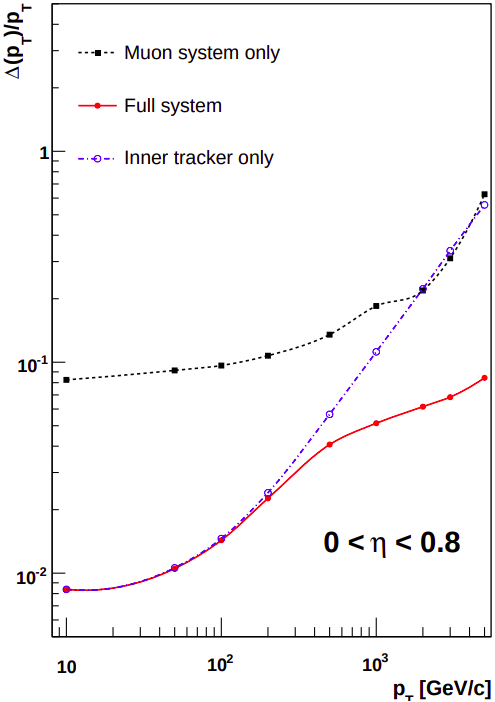
\includegraphics[width=0.5\textwidth]{Figures/muon_res_loweta.png}}
    \subfloat[]{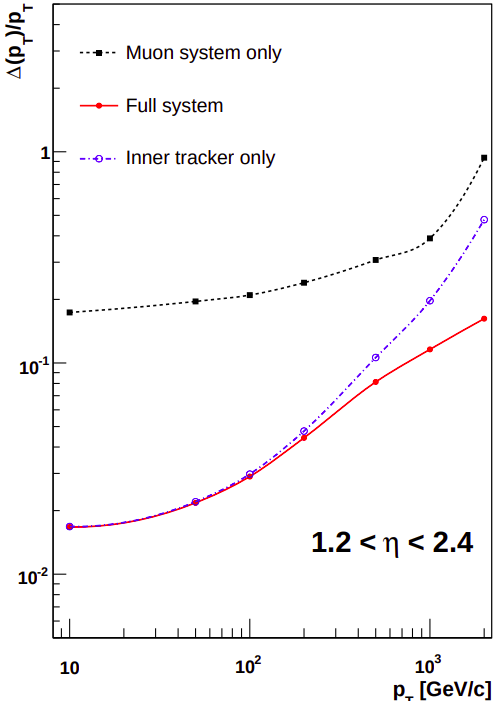
\includegraphics[width=0.5\textwidth]{Figures/muon_res_higheta.png}} \\
\caption{The $\pT$ resolution for muon identification using the muon system (black), the inner tracker (blue), and the full system (red). This is shown for the pseduorapidity regions $0 < \eta < 0.8$ (a) and  $1.2 < \eta < 2.4$ (b)}
\label{fig:muon_eff}
\end{figure}

\section{Electrons}

In addition, electrons are required to pass an identification variable based on a Boosted Decision Tree (BDT) 
discriminator which uses track quality, shower shapes and kinematic quantities as input.
The following variables are used as input to the BDT:  ~\cite{cmsElectron}
\begin{itemize}
\item Cluster shape variables $\sigma_{i\eta,i\eta}$ and $\sigma_{i\phi,i\phi}$, with $i\eta$ and $i\phi$ the integer
label of the $\eta$ and $\phi$ calorimeter cell. The circularity =  $1 -\frac{E1\times5}{E5\times5}$, with
$E1\times5$ and $E5\times5$ the energies in a $1\times5$ and a $5\times5$ grid around the super cluster seed,
respectively. Shape variable R9 = $\frac{E3\times3}{E_{SC}}$, with $E3\times3$ the energy in a $3\times3$ grid
of cells around the super cluster seed and $E_{SC}$ the raw energy of the super cluster.
\item The number of valid hits in the track fit, the $\chi^2$ of the track fit and the $\chi^2$ of the GSFTrack fit
\item The number of GSFtrack hits, the number of expected missing inner hits and the result of the conversion vertex fit
\item The distance $\Delta \eta$ and $\Delta \phi$ between the reconstructed super cluster and the associated track at the position of the primary vertex, and the distance in $\eta$ between the super cluster and the track at the calorimeter surface.
\item H/E, the ratio of the hadronic energy over the electromagnetic energy in the super cluster and E/P, the ratio of the super cluster energy over the momentum of the track associated with the electron 
\item The ratio of the energy of the electron cluster and the momentum of the associated track, evaluated at the electron cluster,
 and $1/E_e - 1/P_e$, with $E_e$ the energy of the electron candidate and $P_e$ its momentum.
\end{itemize}
The BDT was trained on a $Z/\gamma^{*}$ Monte Carlo sample generated with
\texttt{MadGraph 5}, in 3 $\eta$ bins for electrons with $p_{\text{T}}>10$ GeV.
This analysis uses the version of the ID BDT without the isolation included in
the training, instead using an additional cut on the electron isolation. This
was shown to give similar performance to the version of the ID including the
isolation and makes defining side-band regions used for estimation of
backgrounds simpler.

The electron are additionally required to pass the 90\% efficiency working point. Finally electrons are also subject to the same impact parameter requirements as the
muons: the impact parameters $d_{xy}$ and $d_{z}$ between the electron track 
and the primary vertex are restricted as $d_{xy}<0.045$~cm and $d_{z}<0.2$~cm to
ensure the electron is associated with the primary vertex.

The isolation used is based on photon and neutral/charged hadron particle flow
candidates within a cone size of $\Delta R<0.3$ of the selected electron but
used a different method to estimate the neutral particles due to pileup, namely
the rho--effective-area method. The pileup in this method is estimated as
$PU=\rho\cdot\text{EA}$, where $\rho$ is the event-specific average pile-up
energy density per unit area in the $\phi$-$\eta$ plane and the EA is the
effective area specific to the given type of isolation. The rho--effective-area
subtracted relative combined isolation variable is defined as:
\begin{equation}
\label{eqn:electron_reliso_rho} 
I_{\text{rel}}^{e} = \frac{\Sigma
    P_{T}(\text{charged}) + \mathrm{max}(\Sigma E_{T}(\text{neutral}) + \Sigma
E_{T}(\text{photon}) - \rho\cdot\text{EA},0)}{P_{T}^{e}}, \end{equation} where
the $\text{EA}$ is measured in bins of $\eta$ as listed in Table
\ref{tab:EleEA}. The electron isolation used is $I_{rel}<0.15$. 

\begin{table}[htb]
\begin{center}
{\footnotesize
\begin{tabular}{|c|c|}
\hline
$\eta$ range & EA \\
\hline
0.0$\leq\eta<$1.0   &  0.1440 \\
1.0$\leq\eta<$1.479 &  0.1562 \\
1.479$\leq\eta<$2.0 &  0.1032 \\
2.0$\leq\eta<$2.2   &  0.0859 \\
2.2$\leq\eta<$2.3   &  0.1116 \\
2.3$\leq\eta<$2.4   &  0.1321 \\
2.4$\leq\eta<$5.0   &  0.1654 \\
\hline
\end{tabular}
} % end footnotesize
\end{center}
\caption{
 Electron effective areas used for the $\rho$-corrected isolation computation.
}
\label{tab:EleEA}
\end{table}

\section{Jets}

Jets are clustered from all particle flow 
candidates using the anti $k_{\text{T}}$ algorithm~\cite{Cacciari:2011ma} with a cone size parameter R=0.4. To reduce the contribution of jets that originate from 
pile--up vertices, charged hadrons that are not associated with the hard--scattering primary vertex are removed from the particle flow candidates 
that form the input to the anti-$k_{\text{T}}$-algorithm (charged hadron subtraction).

Practically, this means we use the "slimmedJets" collection from the miniAOD dataformat, 
where the jet-energy corrections from global tags

The jets are required to pass the tight working point of
the PF jet ID discriminator provided by the jetMET POG~\cite{PFJetID}.  
To exclude selected $e,\mu,\tau_{h}$ candidates from the jet collection, the jets
are required to be separated from the selected $\tau$ candidate by $\Delta R
> 0.5$.  Jets with a corrected $p_{\text{T}} > 30$ GeV and $|\eta|<4.7$ are
considered.

High endcap ECAL noise in 2017 led to large amounts of noise in reconstructed jets~\cite{JetTwiki}. To mitigate the noise issue,
jets reconstructed on 2017 data also used a veto of jets with
raw $p_{t} < 50$ and $2.65 < |\eta| < 3.139$. 

\section{b jets}

For determining information about the b-tagging status of the jets, the
\texttt{DeepJet} algorithm~\cite{DeepFlavour} is used.  Jets with $p_{\text{T}} > 20$ and $|\eta| < 2.4 (2.5)$ in 2016 (2017 and 2018) are considered
b-tagged if their discriminator value is larger than 0.3093, 0.3033 or 
0.2770 in the 2016, 2017 or 2018 analysis, respectively. This
corresponds to the medium working point provided by the BTV POG
~\cite{BTVPOG_2016,BTVPOG_2017,BTVPOG_2018}.

\section{Missing transverse energy}

The missing transverse energy in the event is reconstructed using the PUPPI algorithm~\cite{CMS-PAS-JME-18-001}, which is more robust towards pileup compared to PF MET, which tends to increase for Run 2 analyses. 
This algorithm is an extension of the PFCHS algorithm and assigns weights to PF candidates
based on the probability that they come from pileup or the primary vertex. Type-I corrections
are applied to correct the MET estimated in this way for over- or underestimation due to inefficiencies in the detector.
These corrections entail the propagation of the JECs to the MET as
\begin{equation}\label{eqn:met_t1corr} \vec{E}_{\text{T}}^{\text{miss,corr}} = \vec{E}_{\text{T}}^{\text{miss}} - \Sigma_{\text{jets}}(\vec{p}_{\text{T}}^{\text{corr}} - \vec{p}_{\text{T}}). \end{equation}


\section{Taus}

Fundamental to this thesis is the identification of tau particles.
The tau lepton is measured to have a mean lifetime of \(2.9 \times 10^{-13}\)s. 
This short lifetimes means that the tau lepton is not directly observable in the \ac{CMS} detector.  
In order to detect these particles, it is important to understand how the tau decays. 
Due to the heavy nature of the particle, it does not only decay leptonically, but unlike the muon, it can also decay hadronically.
A list of prominent decays of the tau lepton are shown in the Tab.~\ref{tab:tau_decay}.
These decays can be split into three groups: the 17.8\% of taus that decay to an electron ($e$), the 17.4\% that decay into a muon ($\mu$), and hadronic tau decays ($\tauh$) that make up the final 64.8\% of tau decays. 
The leptonic decays of the tau can be accounted for by the identification of electrons and muons as discussed in the previous subsection.  \\

\begin{table}[h]
    \centering
    \begin{tabular}{|c|c|}
         \hline
         Decay Mode & Branching Fraction  \\
         \hline
         \hline
         \textbf{Leptonic Decay ($e$, $\mu$)} & \textbf{35.2\%} \\
         $e^- \bar{\nu}_e \nu_\tau $ & 17.8\% \\
         $\mu^- \bar{\nu}_\mu \nu_\tau $ & 17.4\% \\
         \hline
         \textbf{Hadronic Decay ($\tauh$)} & \textbf{64.8\%} \\
         $h^- \pi^0 \nu_\tau $ & 25.9\% \\
         $h^- \nu_\tau$ & 11.5\% \\
         $h^- h^+ h^+ \nu_\tau$ & 9.8\% \\
         $h^- 2\pi^0 \nu_\tau$ & 9.3\% \\
         $h^- h^+ h^- \pi^0 \nu_\tau$ & 4.8\% \\
         other & 3.2\% \\
         \hline
    \end{tabular}
    \caption{Measured branching fractions for the tau lepton. h represents a charged hadron either a pion or a kaon~\cite{ParticleDataGroup:2022pth}.}
    \label{tab:tau_decay}
\end{table}

A two step process is used to identify hadronic taus.
The \ac{HPS} algorithm is used to initially identify hadronic taus based on jets produced by the anti-$k_{\text{T}}$ algorithm with a distance parameter of $\Delta R = 0.4$. 
To capture the energy deposits left by $\pi^0$ candidates in the ECAL, the photon and electron constituents of the jet responsible for seeding the tau reconstruction are assembled into strips. 
All electrons or photons used are required to have $p_{\text{T}} > 0.5$ GeV.
The initial iteration of the \ac{HPS} algorithm used a fixed strip size of $\Delta \eta \times \Delta \phi$ equal to $0.05 \times 0.20$.
However, this technique was updated to a dynamical strip size to account for the multiple scatterings of $e^+ e^-$ products from a $pi^0$ decay, falling outside of the fixed window.
A reliance of the hadronic tau $\pT$ spectrum of the required strip size was observed and so the following iterative algorithm was proposed to resolve this issue.

\begin{enumerate}[i)]
\item The highest $\pT$ electron or photon (not previously grouped into a strip) is used to initiate a new strip.
\item The second highest $\pT$ electron or photon deposition within,
\begin{equation}
  \Delta \eta = f(\pT^{e/\gamma}) + f(\pT^{\text{strip}}), \hspace{1cm} \Delta \phi = g(\pT^{e/\gamma}) + g(\pT^{\text{strip}})
\end{equation}
of the strip is then combined with the strip.
These functions are determined from a fit to hadronic tau MC, so that 95\% of electrons and photons are contained in a single strip.
These fits are shown in Fig.~\ref{fig:hps} and correspond to,
\begin{equation}
f(\pT) = 0.20 \pT^{-0.66}, \hspace{1cm} g(\pT) = 0.35 \pT^{-0.71}
\end{equation}
where the $\pT$ is in units of GeV.
These functions have lower and upper caps of 0.05 to 0.3 for $\Delta\phi$ and 0.05 to 0.15 for $\Delta\eta$.
\item Recalculate the strip position using a weight average of the average $\pT$ of all the electron and photon strip constituents.
\begin{equation}
\eta_{\text{strip}} = \frac{1}{\pT^{\text{strip}}} \sum \pT^{e/\gamma} \eta_{e/\gamma}, \hspace{1cm} \phi_{\text{strip}} = \frac{1}{\pT^{\text{strip}}} \sum \pT^{e/\gamma} \phi_{e/\gamma}
\end{equation}
\item Repeat steps ii and iii until no other electron or photon candidate fulfilling condition ii is found.
\end{enumerate}

\begin{figure}[!hbtp]
\centering
    \subfloat[]{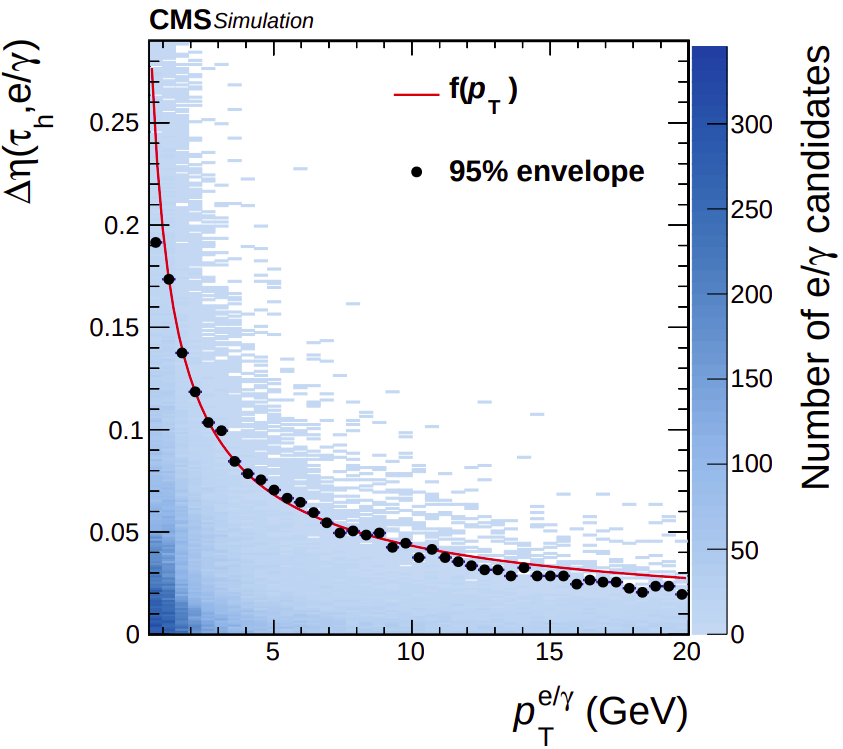
\includegraphics[width=0.5\textwidth]{Figures/hps_f.png}}
    \subfloat[]{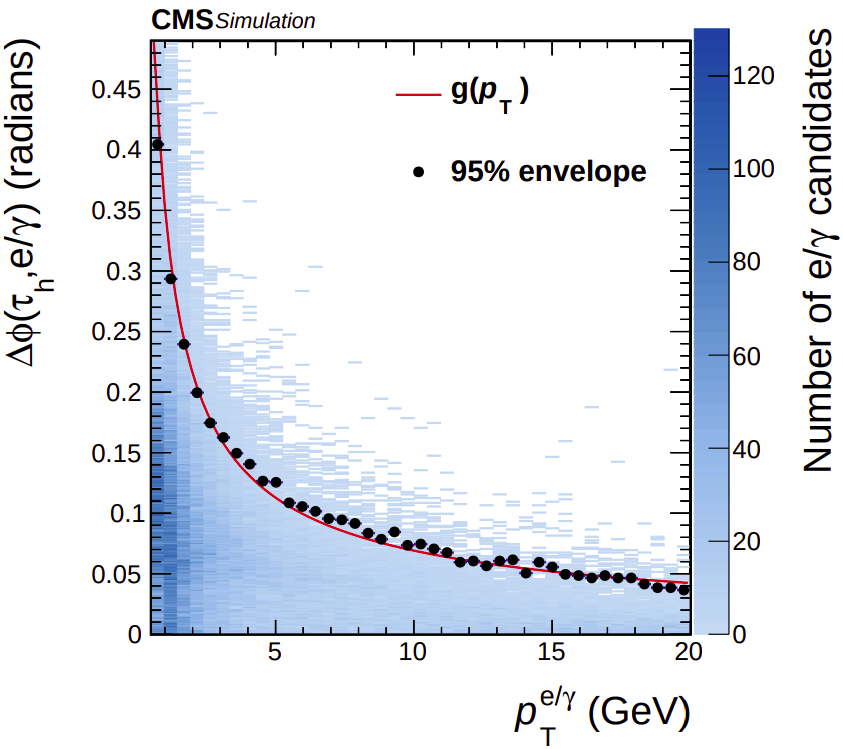
\includegraphics[width=0.5\textwidth]{Figures/hps_g.png}} \\
\caption{The distance between the hadronic tau and electron or photon $\eta$ (a) and $\phi$ (b) with respect the the electron or photon $\pT$. The binned values (points) and the fitted functions $f$ and $g$ (red line), that encapsulates 95\% of all electron and photons are shown in both cases~\cite{Sirunyan:2018pgf}.}
\label{fig:hps}
\end{figure}

Charged hadrons (prongs) are also required to have $\pT > 0.5$ GeV and originate from the \ac{PV}, with a loose transverse impact parameter of $d_{xy} < 0.1$ cm
Further constraints are placed on the reconstructed masses of the specific resonances produced by a hadronic tau decay, if produced by the decay.
In particular, the visible mass positions and widths of the grouped charged hadrons and strips are optimised to match the $\rho$ (770 MeV) and $a_1$ (1260 MeV) decays.
This is performed to maximise the fraction of hadronic tau efficiency to the probability of misidentification from jets.
The visible decay products of each decay shown in Tab~\ref{tab:tau_decay} are reconstructed by:

\begin{enumerate}[i)]
\item $h^- \pi^0$: One charged hadron candidate and no strips.
\item $h^-$: One charged hadron candidate and one strip with mass $ 0.3 < m_{\tau} < 1.3 \sqrt{p_{\text{T}}/100}$ GeV. The mass is required to be between 1.3 and 4.2 GeV.
\item $\pi^- \pi^- \pi^+$: Three charged hadron candidates with mass $0.8 < m_{\tau} < 1.5$ GeV. The tracks are required to originate within $\Delta z<0.4$ cm of the same vertex.
\item $h^- 2\pi^0$: One charged hadron candidate and two strips. The $\tau_{h}$ mass should be $0.4 < m_{\tau} < 1.2\sqrt{p_{\text{T}}/100}$~GeV. The mass is required to be between 1.2 and 4.0 GeV.
\item $\pi^- \pi^- \pi^+ \pi^0$: Three charged hadron candidates and one strip.
\end{enumerate}

The remaining hadronic decays of the tau leptons are not included in this thesis.
The \ac{DM} of the hadronic tau that is reconstructed by a \ac{HPS} is quantified by the following formula relating the number of charged hadron candidates $N_C$ and the number of strips $N_N$.

\begin{equation}
\text{DM} = 5(N_{C} - 1) + N_{N}
\end{equation}

The second step of the identification, comes from a multiclass \ac{DNN}-based algorithm named \texttt{DeepTau}, that seeks to discriminate hadronic tau decays from electron, muons, and most importantly quark or gluon jets, that can be misidentified as hadronic tau decays~\cite{CMS:2022prd}.
It uses a \ac{DNN} architecture that consists of multiple interconnected layers of nodes, that attempts to learn whether the input object is an hadronic tau decay, an electron, a muon or a jet. 
The algorithm takes inputs from reconstructed particles surrounding the \ac{HPS} hadronic tau candidate, including information about energies, momenta, and spatial positions. 
Convolutional layers are used to efficiently process these inputs by dividing them into smaller regions in $\eta$-$\phi$ space, which allows the algorithm to extract local patterns and features. 
It also incorporates high-level features of the hadronic tau candidate calculated from the \ac{HPS} algorithm, such as the four-momentum, charge, \ac{DM}, isolation variables used in previous \ac{MVA}~\cite{CMS:2018jrd}, impact parameters, $\eta$ and $\phi$ strip information, as well as event level information such as variables related to the $\ac{PU}$.
The architecture of algorithm is shown in Fig.~\ref{fig:deeptau}. \\

\begin{figure}[!hbtp]
\centering
    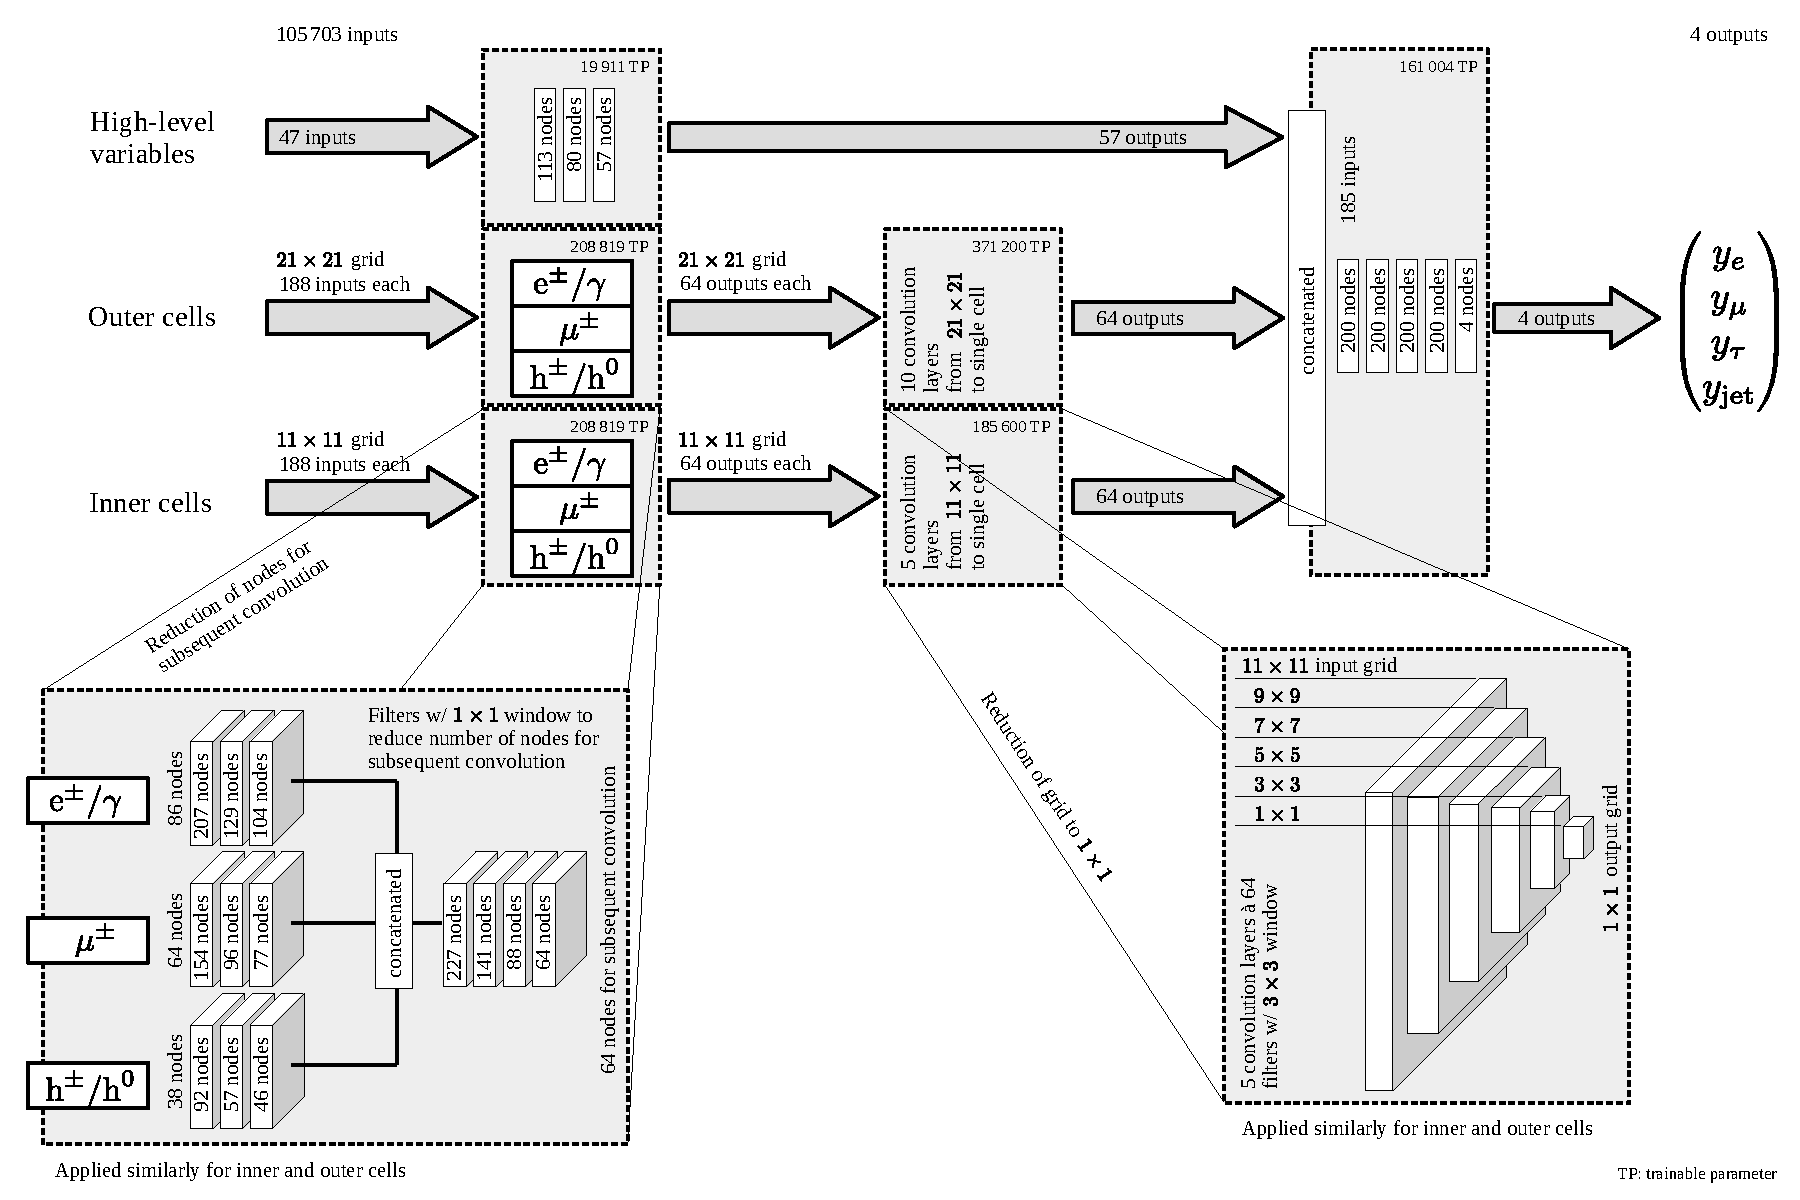
\includegraphics[width=\textwidth]{Figures/deeptau.pdf}
\caption{The architecture of the \texttt{DeepTau} neural network~\cite{CMS:2022prd}. The architecture comprises three sets of input variables: inner cells, outer cells, and high-level features. These sets are processed separately through subnetworks and their outputs are concatenated. Five fully connected layers process the concatenated output to calculate the probabilities for a candidate to be a hadronic tau, electron, muon, or jet. The high-level input subnetwork consists of three fully connected layers, taking 47 inputs and yielding 57 outputs. Complex subnetworks process the features of inner and outer cells separately, with fully connected layers followed by concatenation and additional fully connected layers. Convolutional layers progressively reduce the grid size for both inner and outer cells. For inner cells, there are 5 convolutional layers, while for outer cells, there are 10 convolutional layers. The number of trainable parameters (TP) for the different subnetworks are also provided.}
\label{fig:deeptau}
\end{figure}

The \texttt{DeepTau} \ac{DNN} is trained using a large dataset, incorporating examples of hadronic tau decays and background processes of electrons, muons and jets. 
The output of the \ac{DNN} is 4 scores, that represent the probability that the object is a hadronic tau ($y_\tau$), an electon ($y_e$), a muon ($y_\mu$) or a jet ($y_{\text{jet}}$).
